\documentclass[a4paper,12pt]{article}
\usepackage[margin=18mm]{geometry}
\usepackage{tikz}
\usepackage{amsmath}
\newcommand{\pFourCell}[2]{\makebox[#1em][c]{\ensuremath{#2}}}
\pagestyle{empty}
\begin{document}
\section*{Spaltentreue LaTeX-Ausgabe}
\noindent Gleichung: \texttt{2*sqrt((x+3)/(2+1))=5} \hfill Zielvariable: \texttt{x} \hfill Profil: \texttt{standard}

\vspace{8mm}
\begin{center}
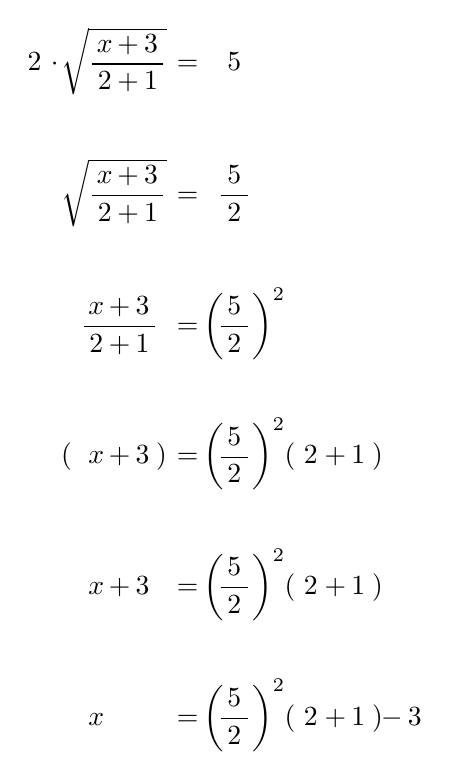
\begin{tikzpicture}[x=1em,y=-1em]
\node[anchor=base, inner sep=0pt] at (0.44,2.9) {$2$};
\node[anchor=base, inner sep=0pt] at (1.17,2.9) {$\cdot$};
\node[anchor=base, inner sep=0pt] at (3.31,2.9) {$\pFourCell{2.94}{\sqrt{\displaystyle\frac{\pFourCell{0.9}{x}\pFourCell{0.78}{+}\pFourCell{0.88}{3}}{\pFourCell{0.9}{2}\pFourCell{0.78}{+}\pFourCell{0.88}{1}}}}$};
\node[anchor=base, inner sep=0pt] at (5.97,2.9) {$=$};
\node[anchor=base, inner sep=0pt] at (7.66,2.9) {$5$};
\node[anchor=base, inner sep=0pt] at (7.66,7.65) {$\displaystyle\frac{\pFourCell{1}{5}}{\pFourCell{1}{2}}$};
\node[anchor=base, inner sep=0pt] at (3.31,7.65) {$\pFourCell{2.94}{\sqrt{\displaystyle\frac{\pFourCell{0.9}{x}\pFourCell{0.78}{+}\pFourCell{0.88}{3}}{\pFourCell{0.9}{2}\pFourCell{0.78}{+}\pFourCell{0.88}{1}}}}$};
\node[anchor=base, inner sep=0pt] at (5.97,7.65) {$=$};
\node[anchor=base, inner sep=0pt] at (3.5,12.385) {$\displaystyle\frac{\pFourCell{0.9}{x}\pFourCell{0.78}{+}\pFourCell{0.88}{3}}{\pFourCell{0.9}{2}\pFourCell{0.78}{+}\pFourCell{0.88}{1}}$};
\node[anchor=base, inner sep=0pt] at (5.97,12.385) {$=$};
\node[anchor=base, inner sep=0pt] at (7.66,12.385) {$\displaystyle\frac{\pFourCell{1}{5}}{\pFourCell{1}{2}}$};
\node[anchor=base, inner sep=0pt] at (6.97,12.385) {$\pFourCell{0.38}{\left(\vphantom{\displaystyle\frac{\pFourCell{1}{5}}{\pFourCell{1}{2}}}\right.}$};
\node[anchor=base, inner sep=0pt] at (8.85,12.385) {$\pFourCell{1.38}{\left.\vphantom{\displaystyle\frac{\pFourCell{1}{5}}{\pFourCell{1}{2}}}\right)^{2}}$};
\node[anchor=base, inner sep=0pt] at (3.5,17.105) {$\pFourCell{0.9}{x}\pFourCell{0.78}{+}\pFourCell{0.88}{3}$};
\node[anchor=base, inner sep=0pt] at (1.65,17.105) {$\pFourCell{0.38}{\left(\vphantom{\pFourCell{0.9}{x}\pFourCell{0.78}{+}\pFourCell{0.88}{3}}\right.}$};
\node[anchor=base, inner sep=0pt] at (4.97,17.105) {$\pFourCell{0.38}{\left.\vphantom{\pFourCell{0.9}{x}\pFourCell{0.78}{+}\pFourCell{0.88}{3}}\right)}$};
\node[anchor=base, inner sep=0pt] at (5.97,17.105) {$=$};
\node[anchor=base, inner sep=0pt] at (7.66,17.105) {$\displaystyle\frac{\pFourCell{1}{5}}{\pFourCell{1}{2}}$};
\node[anchor=base, inner sep=0pt] at (6.97,17.105) {$\pFourCell{0.38}{\left(\vphantom{\displaystyle\frac{\pFourCell{1}{5}}{\pFourCell{1}{2}}}\right.}$};
\node[anchor=base, inner sep=0pt] at (8.85,17.105) {$\pFourCell{1.38}{\left.\vphantom{\displaystyle\frac{\pFourCell{1}{5}}{\pFourCell{1}{2}}}\right)^{2}}$};
\node[anchor=base, inner sep=0pt] at (11.25,17.105) {$\pFourCell{1}{2}\pFourCell{0.78}{+}\pFourCell{0.88}{1}$};
\node[anchor=base, inner sep=0pt] at (9.73,17.105) {$\pFourCell{0.38}{\left(\vphantom{\pFourCell{1}{2}\pFourCell{0.78}{+}\pFourCell{0.88}{1}}\right.}$};
\node[anchor=base, inner sep=0pt] at (12.77,17.105) {$\pFourCell{0.38}{\left.\vphantom{\pFourCell{1}{2}\pFourCell{0.78}{+}\pFourCell{0.88}{1}}\right)}$};
\node[anchor=base, inner sep=0pt] at (2.67,21.825) {$x$};
\node[anchor=base, inner sep=0pt] at (3.51,21.825) {$+$};
\node[anchor=base, inner sep=0pt] at (4.34,21.825) {$3$};
\node[anchor=base, inner sep=0pt] at (5.97,21.825) {$=$};
\node[anchor=base, inner sep=0pt] at (7.66,21.825) {$\displaystyle\frac{\pFourCell{1}{5}}{\pFourCell{1}{2}}$};
\node[anchor=base, inner sep=0pt] at (6.97,21.825) {$\pFourCell{0.38}{\left(\vphantom{\displaystyle\frac{\pFourCell{1}{5}}{\pFourCell{1}{2}}}\right.}$};
\node[anchor=base, inner sep=0pt] at (8.85,21.825) {$\pFourCell{1.38}{\left.\vphantom{\displaystyle\frac{\pFourCell{1}{5}}{\pFourCell{1}{2}}}\right)^{2}}$};
\node[anchor=base, inner sep=0pt] at (11.25,21.825) {$\pFourCell{1}{2}\pFourCell{0.78}{+}\pFourCell{0.88}{1}$};
\node[anchor=base, inner sep=0pt] at (9.73,21.825) {$\pFourCell{0.38}{\left(\vphantom{\pFourCell{1}{2}\pFourCell{0.78}{+}\pFourCell{0.88}{1}}\right.}$};
\node[anchor=base, inner sep=0pt] at (12.77,21.825) {$\pFourCell{0.38}{\left.\vphantom{\pFourCell{1}{2}\pFourCell{0.78}{+}\pFourCell{0.88}{1}}\right)}$};
\node[anchor=base, inner sep=0pt] at (2.67,26.545) {$x$};
\node[anchor=base, inner sep=0pt] at (5.97,26.545) {$=$};
\node[anchor=base, inner sep=0pt] at (7.66,26.545) {$\displaystyle\frac{\pFourCell{1}{5}}{\pFourCell{1}{2}}$};
\node[anchor=base, inner sep=0pt] at (6.97,26.545) {$\pFourCell{0.38}{\left(\vphantom{\displaystyle\frac{\pFourCell{1}{5}}{\pFourCell{1}{2}}}\right.}$};
\node[anchor=base, inner sep=0pt] at (8.85,26.545) {$\pFourCell{1.38}{\left.\vphantom{\displaystyle\frac{\pFourCell{1}{5}}{\pFourCell{1}{2}}}\right)^{2}}$};
\node[anchor=base, inner sep=0pt] at (11.25,26.545) {$\pFourCell{1}{2}\pFourCell{0.78}{+}\pFourCell{0.88}{1}$};
\node[anchor=base, inner sep=0pt] at (9.73,26.545) {$\pFourCell{0.38}{\left(\vphantom{\pFourCell{1}{2}\pFourCell{0.78}{+}\pFourCell{0.88}{1}}\right.}$};
\node[anchor=base, inner sep=0pt] at (12.77,26.545) {$\pFourCell{0.38}{\left.\vphantom{\pFourCell{1}{2}\pFourCell{0.78}{+}\pFourCell{0.88}{1}}\right)}$};
\node[anchor=base, inner sep=0pt] at (13.35,26.545) {$-$};
\node[anchor=base, inner sep=0pt] at (14.18,26.545) {$3$};
\end{tikzpicture}
\end{center}

\newpage
\section*{Spaltentreue LaTeX-Ausgabe mit Spaltengrenzen}
\vspace{6mm}
\begin{center}
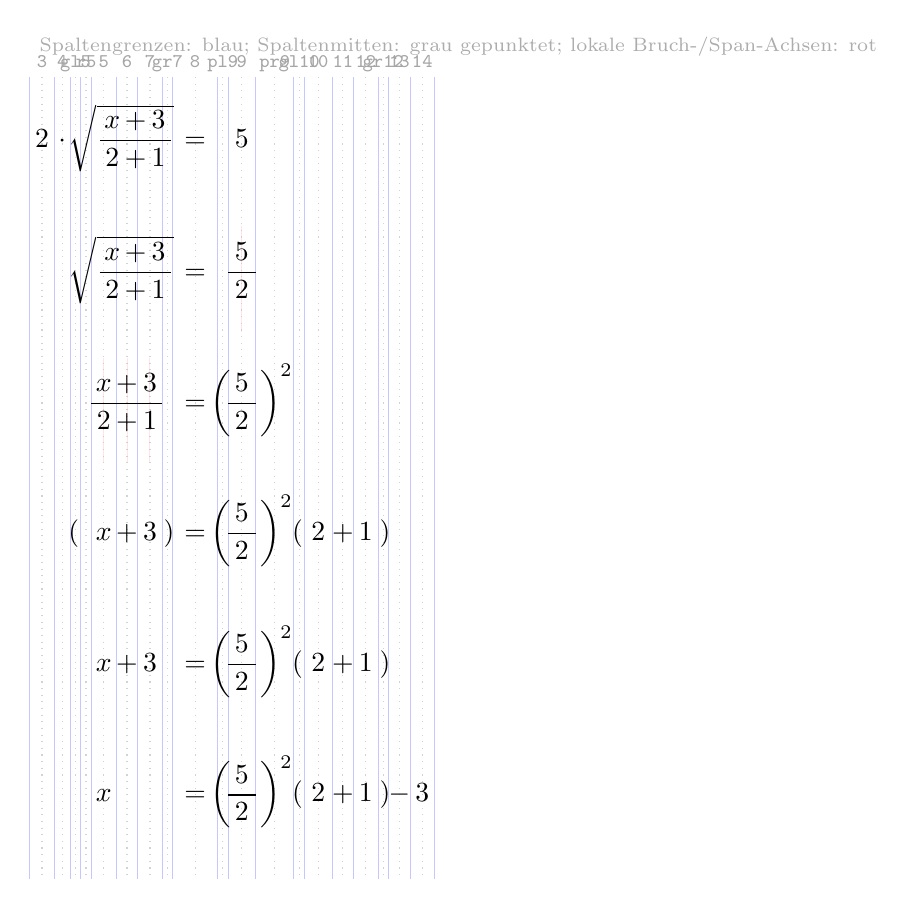
\begin{tikzpicture}[x=1em,y=-1em]
\node[font={\scriptsize}, text=gray!65, anchor=west] at (0,-0.75) {Spaltengrenzen: blau; Spaltenmitten: grau gepunktet; lokale Bruch-/Span-Achsen: rot};
\draw[blue!22, line width=0.28pt] (0,0.35) -- (0,29.33);
\draw[blue!22, line width=0.28pt] (0.88,0.35) -- (0.88,29.33);
\draw[blue!22, line width=0.28pt] (1.46,0.35) -- (1.46,29.33);
\draw[blue!22, line width=0.28pt] (1.84,0.35) -- (1.84,29.33);
\draw[blue!22, line width=0.28pt] (2.22,0.35) -- (2.22,29.33);
\draw[blue!22, line width=0.28pt] (3.12,0.35) -- (3.12,29.33);
\draw[blue!22, line width=0.28pt] (3.9,0.35) -- (3.9,29.33);
\draw[blue!22, line width=0.28pt] (4.78,0.35) -- (4.78,29.33);
\draw[blue!22, line width=0.28pt] (5.16,0.35) -- (5.16,29.33);
\draw[blue!22, line width=0.28pt] (6.78,0.35) -- (6.78,29.33);
\draw[blue!22, line width=0.28pt] (7.16,0.35) -- (7.16,29.33);
\draw[blue!22, line width=0.28pt] (8.16,0.35) -- (8.16,29.33);
\draw[blue!22, line width=0.28pt] (9.54,0.35) -- (9.54,29.33);
\draw[blue!22, line width=0.28pt] (9.92,0.35) -- (9.92,29.33);
\draw[blue!22, line width=0.28pt] (10.92,0.35) -- (10.92,29.33);
\draw[blue!22, line width=0.28pt] (11.7,0.35) -- (11.7,29.33);
\draw[blue!22, line width=0.28pt] (12.58,0.35) -- (12.58,29.33);
\draw[blue!22, line width=0.28pt] (12.96,0.35) -- (12.96,29.33);
\draw[blue!22, line width=0.28pt] (13.74,0.35) -- (13.74,29.33);
\draw[blue!22, line width=0.28pt] (14.62,0.35) -- (14.62,29.33);
\draw[gray!35, dotted] (0.44,0.35) -- (0.44,29.33);
\node[font={\ttfamily\scriptsize}, text=gray!70, anchor=base] at (0.44,0) {3};
\draw[gray!35, dotted] (1.17,0.35) -- (1.17,29.33);
\node[font={\ttfamily\scriptsize}, text=gray!70, anchor=base] at (1.17,0) {4};
\draw[gray!35, dotted] (1.65,0.35) -- (1.65,29.33);
\node[font={\ttfamily\scriptsize}, text=gray!70, anchor=base] at (1.65,0) {gl5};
\draw[gray!35, dotted] (2.03,0.35) -- (2.03,29.33);
\node[font={\ttfamily\scriptsize}, text=gray!70, anchor=base] at (2.03,0) {r5};
\draw[gray!35, dotted] (2.67,0.35) -- (2.67,29.33);
\node[font={\ttfamily\scriptsize}, text=gray!70, anchor=base] at (2.67,0) {5};
\draw[gray!35, dotted] (3.51,0.35) -- (3.51,29.33);
\node[font={\ttfamily\scriptsize}, text=gray!70, anchor=base] at (3.51,0) {6};
\draw[gray!35, dotted] (4.34,0.35) -- (4.34,29.33);
\node[font={\ttfamily\scriptsize}, text=gray!70, anchor=base] at (4.34,0) {7};
\draw[gray!35, dotted] (4.97,0.35) -- (4.97,29.33);
\node[font={\ttfamily\scriptsize}, text=gray!70, anchor=base] at (4.97,0) {gr7};
\draw[gray!35, dotted] (5.97,0.35) -- (5.97,29.33);
\node[font={\ttfamily\scriptsize}, text=gray!70, anchor=base] at (5.97,0) {8};
\draw[gray!35, dotted] (6.97,0.35) -- (6.97,29.33);
\node[font={\ttfamily\scriptsize}, text=gray!70, anchor=base] at (6.97,0) {pl9};
\draw[gray!35, dotted] (7.66,0.35) -- (7.66,29.33);
\node[font={\ttfamily\scriptsize}, text=gray!70, anchor=base] at (7.66,0) {9};
\draw[gray!35, dotted] (8.85,0.35) -- (8.85,29.33);
\node[font={\ttfamily\scriptsize}, text=gray!70, anchor=base] at (8.85,0) {pr9};
\draw[gray!35, dotted] (9.73,0.35) -- (9.73,29.33);
\node[font={\ttfamily\scriptsize}, text=gray!70, anchor=base] at (9.73,0) {gl10};
\draw[gray!35, dotted] (10.42,0.35) -- (10.42,29.33);
\node[font={\ttfamily\scriptsize}, text=gray!70, anchor=base] at (10.42,0) {10};
\draw[gray!35, dotted] (11.31,0.35) -- (11.31,29.33);
\node[font={\ttfamily\scriptsize}, text=gray!70, anchor=base] at (11.31,0) {11};
\draw[gray!35, dotted] (12.14,0.35) -- (12.14,29.33);
\node[font={\ttfamily\scriptsize}, text=gray!70, anchor=base] at (12.14,0) {12};
\draw[gray!35, dotted] (12.77,0.35) -- (12.77,29.33);
\node[font={\ttfamily\scriptsize}, text=gray!70, anchor=base] at (12.77,0) {gr12};
\draw[gray!35, dotted] (13.35,0.35) -- (13.35,29.33);
\node[font={\ttfamily\scriptsize}, text=gray!70, anchor=base] at (13.35,0) {13};
\draw[gray!35, dotted] (14.18,0.35) -- (14.18,29.33);
\node[font={\ttfamily\scriptsize}, text=gray!70, anchor=base] at (14.18,0) {14};
\node[anchor=base, inner sep=0pt] at (0.44,2.9) {$2$};
\node[anchor=base, inner sep=0pt] at (1.17,2.9) {$\cdot$};
\node[anchor=base, inner sep=0pt] at (3.31,2.9) {$\pFourCell{2.94}{\sqrt{\displaystyle\frac{\pFourCell{0.9}{x}\pFourCell{0.78}{+}\pFourCell{0.88}{3}}{\pFourCell{0.9}{2}\pFourCell{0.78}{+}\pFourCell{0.88}{1}}}}$};
\node[anchor=base, inner sep=0pt] at (5.97,2.9) {$=$};
\node[anchor=base, inner sep=0pt] at (7.66,2.9) {$5$};
\draw[red!30, opacity=0.32, line width=0.35pt] (7.66,5.75) -- (7.66,9.55);
\node[anchor=base, inner sep=0pt] at (7.66,7.65) {$\displaystyle\frac{\pFourCell{1}{5}}{\pFourCell{1}{2}}$};
\node[anchor=base, inner sep=0pt] at (3.31,7.65) {$\pFourCell{2.94}{\sqrt{\displaystyle\frac{\pFourCell{0.9}{x}\pFourCell{0.78}{+}\pFourCell{0.88}{3}}{\pFourCell{0.9}{2}\pFourCell{0.78}{+}\pFourCell{0.88}{1}}}}$};
\node[anchor=base, inner sep=0pt] at (5.97,7.65) {$=$};
\draw[red!30, opacity=0.32, line width=0.35pt] (2.67,10.5) -- (2.67,14.27);
\draw[red!30, opacity=0.32, line width=0.35pt] (3.51,10.5) -- (3.51,14.27);
\draw[red!30, opacity=0.32, line width=0.35pt] (4.34,10.5) -- (4.34,14.27);
\node[anchor=base, inner sep=0pt] at (3.5,12.385) {$\displaystyle\frac{\pFourCell{0.9}{x}\pFourCell{0.78}{+}\pFourCell{0.88}{3}}{\pFourCell{0.9}{2}\pFourCell{0.78}{+}\pFourCell{0.88}{1}}$};
\node[anchor=base, inner sep=0pt] at (5.97,12.385) {$=$};
\node[anchor=base, inner sep=0pt] at (7.66,12.385) {$\displaystyle\frac{\pFourCell{1}{5}}{\pFourCell{1}{2}}$};
\node[anchor=base, inner sep=0pt] at (6.97,12.385) {$\pFourCell{0.38}{\left(\vphantom{\displaystyle\frac{\pFourCell{1}{5}}{\pFourCell{1}{2}}}\right.}$};
\node[anchor=base, inner sep=0pt] at (8.85,12.385) {$\pFourCell{1.38}{\left.\vphantom{\displaystyle\frac{\pFourCell{1}{5}}{\pFourCell{1}{2}}}\right)^{2}}$};
\node[anchor=base, inner sep=0pt] at (3.5,17.105) {$\pFourCell{0.9}{x}\pFourCell{0.78}{+}\pFourCell{0.88}{3}$};
\node[anchor=base, inner sep=0pt] at (1.65,17.105) {$\pFourCell{0.38}{\left(\vphantom{\pFourCell{0.9}{x}\pFourCell{0.78}{+}\pFourCell{0.88}{3}}\right.}$};
\node[anchor=base, inner sep=0pt] at (4.97,17.105) {$\pFourCell{0.38}{\left.\vphantom{\pFourCell{0.9}{x}\pFourCell{0.78}{+}\pFourCell{0.88}{3}}\right)}$};
\node[anchor=base, inner sep=0pt] at (5.97,17.105) {$=$};
\node[anchor=base, inner sep=0pt] at (7.66,17.105) {$\displaystyle\frac{\pFourCell{1}{5}}{\pFourCell{1}{2}}$};
\node[anchor=base, inner sep=0pt] at (6.97,17.105) {$\pFourCell{0.38}{\left(\vphantom{\displaystyle\frac{\pFourCell{1}{5}}{\pFourCell{1}{2}}}\right.}$};
\node[anchor=base, inner sep=0pt] at (8.85,17.105) {$\pFourCell{1.38}{\left.\vphantom{\displaystyle\frac{\pFourCell{1}{5}}{\pFourCell{1}{2}}}\right)^{2}}$};
\node[anchor=base, inner sep=0pt] at (11.25,17.105) {$\pFourCell{1}{2}\pFourCell{0.78}{+}\pFourCell{0.88}{1}$};
\node[anchor=base, inner sep=0pt] at (9.73,17.105) {$\pFourCell{0.38}{\left(\vphantom{\pFourCell{1}{2}\pFourCell{0.78}{+}\pFourCell{0.88}{1}}\right.}$};
\node[anchor=base, inner sep=0pt] at (12.77,17.105) {$\pFourCell{0.38}{\left.\vphantom{\pFourCell{1}{2}\pFourCell{0.78}{+}\pFourCell{0.88}{1}}\right)}$};
\node[anchor=base, inner sep=0pt] at (2.67,21.825) {$x$};
\node[anchor=base, inner sep=0pt] at (3.51,21.825) {$+$};
\node[anchor=base, inner sep=0pt] at (4.34,21.825) {$3$};
\node[anchor=base, inner sep=0pt] at (5.97,21.825) {$=$};
\node[anchor=base, inner sep=0pt] at (7.66,21.825) {$\displaystyle\frac{\pFourCell{1}{5}}{\pFourCell{1}{2}}$};
\node[anchor=base, inner sep=0pt] at (6.97,21.825) {$\pFourCell{0.38}{\left(\vphantom{\displaystyle\frac{\pFourCell{1}{5}}{\pFourCell{1}{2}}}\right.}$};
\node[anchor=base, inner sep=0pt] at (8.85,21.825) {$\pFourCell{1.38}{\left.\vphantom{\displaystyle\frac{\pFourCell{1}{5}}{\pFourCell{1}{2}}}\right)^{2}}$};
\node[anchor=base, inner sep=0pt] at (11.25,21.825) {$\pFourCell{1}{2}\pFourCell{0.78}{+}\pFourCell{0.88}{1}$};
\node[anchor=base, inner sep=0pt] at (9.73,21.825) {$\pFourCell{0.38}{\left(\vphantom{\pFourCell{1}{2}\pFourCell{0.78}{+}\pFourCell{0.88}{1}}\right.}$};
\node[anchor=base, inner sep=0pt] at (12.77,21.825) {$\pFourCell{0.38}{\left.\vphantom{\pFourCell{1}{2}\pFourCell{0.78}{+}\pFourCell{0.88}{1}}\right)}$};
\node[anchor=base, inner sep=0pt] at (2.67,26.545) {$x$};
\node[anchor=base, inner sep=0pt] at (5.97,26.545) {$=$};
\node[anchor=base, inner sep=0pt] at (7.66,26.545) {$\displaystyle\frac{\pFourCell{1}{5}}{\pFourCell{1}{2}}$};
\node[anchor=base, inner sep=0pt] at (6.97,26.545) {$\pFourCell{0.38}{\left(\vphantom{\displaystyle\frac{\pFourCell{1}{5}}{\pFourCell{1}{2}}}\right.}$};
\node[anchor=base, inner sep=0pt] at (8.85,26.545) {$\pFourCell{1.38}{\left.\vphantom{\displaystyle\frac{\pFourCell{1}{5}}{\pFourCell{1}{2}}}\right)^{2}}$};
\node[anchor=base, inner sep=0pt] at (11.25,26.545) {$\pFourCell{1}{2}\pFourCell{0.78}{+}\pFourCell{0.88}{1}$};
\node[anchor=base, inner sep=0pt] at (9.73,26.545) {$\pFourCell{0.38}{\left(\vphantom{\pFourCell{1}{2}\pFourCell{0.78}{+}\pFourCell{0.88}{1}}\right.}$};
\node[anchor=base, inner sep=0pt] at (12.77,26.545) {$\pFourCell{0.38}{\left.\vphantom{\pFourCell{1}{2}\pFourCell{0.78}{+}\pFourCell{0.88}{1}}\right)}$};
\node[anchor=base, inner sep=0pt] at (13.35,26.545) {$-$};
\node[anchor=base, inner sep=0pt] at (14.18,26.545) {$3$};
\end{tikzpicture}
\end{center}
\end{document}
